\documentclass[11pt]{article}

\usepackage{fullpage}
\usepackage{graphicx}
\usepackage{rotate}
\usepackage{booktabs}
\usepackage{subfigure}

\def\rootdir{../}

\begin{document}

\section*{Lecture aims}

 \begin{enumerate}

 \item Produce a fault-tolerant design (using hardware and software redundancy) that increases the reliability of a system.

 \item Describe and implement several techniques for information redundancy.
 \end{enumerate}

\section*{Lecture plan}
  
\subsubsection*{Introduction}

\begin{enumerate}
  \item Definition of fault tolerance: important to draw the idea that it is about detecting (and maybe correcting) faults in a system so that it can \emph{continue operating correctly} (of safely, securely, etc.).

  \item Fault tolerance recognises that we will make mistakes in producing systems, so we need to work around the,

  \item \emph{Redundancy} is the key to fault tolerance. Four types: hardware, software, information, and time (re-calculation). Only focus on first three.

  \item Hardware vs software failures:

  \begin{itemize}
   \item Hardware fails from manufacturing fault or from wear and tear. For the latter, it fails randomly.
   \item Software fails from design faults, does not wear out. It fails systematically.
  \end{itemize}

 \end{enumerate}

\subsubsection*{Hardware redundancy}

\begin{enumerate}

 \item Show Lardner's quote about redundancy (below). 

 \item Redundancy still key today, however, simply doing re-calculation is not going to work for e.g. software.

 \item Static pairs: calculate answer, if not the same, an \emph{interface} switches off pair from network (draw figure).

 \item Static pairs: what if the interface is faulty? Use a monitor --- monitor and interface check each other (draw figure below).

 \item Static pairs detect failure, but cannot tolerate it. For that, new more than 2 units.... a \emph{voting}.

 \item Approximate vs. exact agreement; \emph{sufficiently equal}

 \item Voting algorithms: majority, k-plurality, and median.

 \item Majority: harder than it sounds.

 \item Majority voting algorithm: group sufficiently equal inputs into classes, take the largest class, $P_i$, and if $\#P_i \geq \frac{N}{2}$, pick any value in $P_i$ as the output. If $\#P_i < \frac{N}{2}$, no agreement.

 \item Use example: 30.1, 30.2, 30.3, 30.5, 30.7, with $\epsilon = 0.2$.

 \item k-plurality: As for majority voting, but $\#P_i \geq k$.

 \item Median voting: take the median. 

 \item Question: why not an \emph{averaging} voter? Faulty measures can influence result.

 \item Question: what if the faulty component is also the median?!

 \item Comparison of voters: show table. Median voters always give output. Majority and k-plurality do not always give output, but are only incorrect under multiple (N or k) failures.

 \item Median voters used when decision is required. Majority or k-plurality used when decision can be delegated.

 \item Architecture: N-modular redundancy. Show figure. Can tolerate $m$ faults with $2M + 1$ components.

\end{enumerate}

\subsubsection*{Software redundancy}

\begin{enumerate}

 \item Software redundancy harder: simply installing $N$ copies of software does not tolerate software failure due to systematic nature of faults.

 \item \emph{N-version programming} is a software-based version of hardware redundancy. Requires that N \emph{independent} versions of the code are written.  All N independent versions of the code are executed and the output is voted on.

 \item Common-mode failures in engineering refer to those failures that are not statistically independent from one another. For example, the back two tires on a car a likely to fail (run out of tread) at around the same time because they will have driven the same distance.

 \item Causes: specification faults, similar development environments, use of similar algorithms, similar training.

 \item Solution: design diversity. Good specification, controlling individual to ensure different tools and algorithms, team separation, different organisations/training.

 \item Does independence work? Show figure from Leveson and Knight (below)

 \item Downsides: common-mode failures exist; cost (re-implement N versions)

 \item Recovery blocks: show figure.

 \item Acceptance tests $\approx$ oracle problem in software testing

 \item Advantages: as we go down the stack, implementations can become simpler: more approximate and less efficient; because they will be executed infrequently.

\end{enumerate}

\subsubsection*{Byzantine failures}

\begin{enumerate}

 \item Malicious/Byzantine failure: different values to multiple units.

 \item Show table of voters below.

 \item Byzantine general's problem (show figures below).

 \item To tolerate $n$ Byzantine failures, we require $3n + 1$ units.

 \item Byzantine algorithm (below): works by essentially have the lieutenants vote by treating each others' orders as votes.

 \item Relation to systems engineering: general is a (possibly faulty) sensor, and lieutenants are (possibly faulty) units

 \item In practice: Lamport's original algorithm too slow. In 2002, Castro and Liskov presented the ``Practical Byzantine Fault Tolerance'' (PBFT) algorithm. Now a flurry of research.

 \item In practice: Bitcoin currency. To obtain a single coin of currency, a node must work as part of a ``proof-of-work'' chain, and synchronisation of the global chain view is performed using a majority vote. Deliberate malicious behaviour tolerated using Byzantine agreement.

\end{enumerate}

\subsubsection*{Information redundancy}

\begin{enumerate}

 \item Duplication. High overhead. Can only detect (unless duplicated twice)

 \item Error detection using parity coding: count 1s and append a single bit.

 \item Interlaced parity coding (show table): example 00000000-1100. Must be bit $w_4$ from table. 

 \item Interlaced parity coding useful for when original data cannot be recovered; e.g. cannot ask to send again; memory storage etc.

 \item Checksums: break up data into words, line up words, and check. Simplest is  \emph{longitudinal parity check}: xor bits in word, then receiver xors  all words \emph{including the checksum}. If the result contains a bit that is non-zero, then an error has been detected.



\end{enumerate}

\pagebreak

\section*{Fault tolerance in practice}

\subsection*{Airbus A310--A380}

The Airbus series of aircraft designs rely heavily on hardware, software, and information redundancy to achieve fault tolerant behaviour of aircraft. 

\begin{enumerate}

 \item A310 (circa 1983) had ten separate digital flight control computers.

 \item A320 (circa 1988) introduced fly by wire, in which four computers teamed in command/monitor pairs for redundancy, which became standard approach for subsequent Airbus flight control computers.

 \item A340 (circa 1992) had one command/monitor pair forming a ``fail fast'' module, failing over to another command/monitor ``hot spare'' pair.  Error detection was achieved through mismatched command, sequence checking, and self-test when aircraft energised.

 A second command/monitor pair using a different microprocessor and different software provided design diversity to tolerate common mode design and manufacturing faults.

 \item A380 (circa 2005) employs dual-redundant Ethernet for non-critical functions, electrical and hydraulic flight control diversity.

 Design diversity in the A380 project was achieved via using dissimilar computers, physical separation of teams, multiple software bases, different software development tools, and data diversity.

\end{enumerate}


\subsection*{Boeing 777}

The Boeing 777 is another aircraft that relies heavily on hardware, software, and information redundancy.

\begin{enumerate}

 \item Goal of Mean Time Between Actions to 25,000 operating hours,
reduce probability of degrading below minimum capability to less
than \(10^{-10}\).

 \item Designed to tolerate Byzantine faults, object impact, component
failure, power failure, electromagnetic interference, cloud
environment.

 \item Byzantine fault tolerance with data synchronisation and median
voting.
 
 \item Architecture of flight control computer has three independent channels each composed of three redundant computing lanes (command, monitor, standby).  Standby allows dispatch of aircraft even with a lane or data channel failure.

 \item Design diversity was achieved using different microprocessor hardware and different software compilers for a fault-intolerant single source code.

\end{enumerate}


\pagebreak

~

~

~

~

~

~

\begin{quote}
``The most certain and effectual check upon errors which arise in the process of computation is to cause the same computations to be made by separate and independent computers; and this check is rendered still more decisive if their computations are carried out by different methods.'' -- D Lardner, 1824.
\end{quote}

\vfill

\begin{center}
 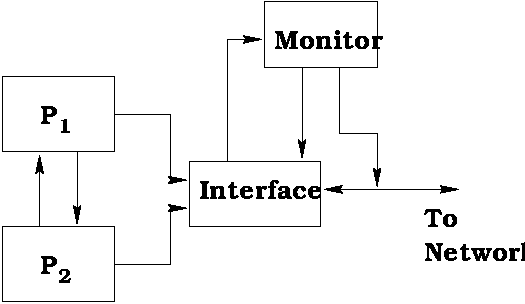
\includegraphics[scale=0.8]{\rootdir/fault-tolerant-design/figures/fault_static_pair}
\end{center}

\vfill

\pagebreak

\begin{center}
\begin{tabular}{llll}
\toprule
{\bf Case} & {\bf Majority} & {\bf \(k\)-plurality} &
             {\bf Median}\\
  & {\bf voter} & {\bf voter} &{\bf voter}\\
\midrule
All outputs correct and SE\(^*\) & Correct & Correct & Correct\\
Majority correct and SE & Correct & Correct & Correct\\
\(k^{\dagger}\) outputs correct and SE 
         & No output & Correct & Possibly correct\\[3mm]
All correct but none SE & No output & No output & Correct\\
All incorrect and none SE & No output & No output & Incorrect\\
\(k^{\dagger}\) outputs incorrect and SE & No output & Incorrect & Possibly correct\\[3mm]
Majority incorrect and SE & Incorrect & Incorrect & Incorrect\\
All incorrect and SE & Incorrect & Incorrect & Incorrect\\
\bottomrule
~\\
\(^*\) SE = Sufficiently equal\\
\(^{\dagger}\) where \(k < \frac{N}{2}\)
\end{tabular}
\end{center}


\vfill

\begin{center}

\end{center}

\vfill
\begin{figure}[!h]
\centering
\subfigure[~]{
  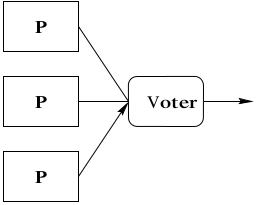
\includegraphics[scale=0.8]{\rootdir/fault-tolerant-design/figures/N-modular-redundancy-single-output}}
~~~
\subfigure[~]{
  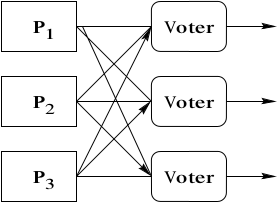
\includegraphics[scale=0.8]{\rootdir/fault-tolerant-design/figures/N-modular-redundancy-multi-outputs}}
\end{figure}

\vfill

\pagebreak

\begin{center}
 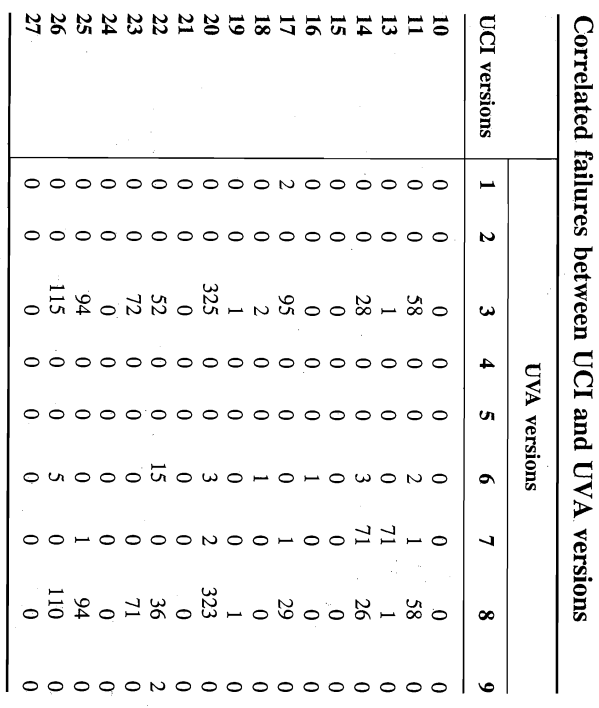
\includegraphics[scale=0.50,angle=90]{\rootdir/fault-tolerant-design/figures/correlated-failures}
\end{center}

\vfill

\begin{center}
 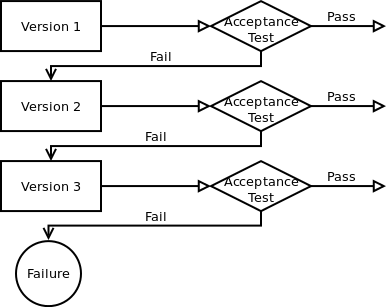
\includegraphics[scale=0.65]{\rootdir/fault-tolerant-design/figures/recovery-blocks}
\end{center}

\vfill 

\pagebreak

\begin{center}
\begin{tabular}{llll}
\hline
 {\bf Sensor} & {\bf Voter 1} & {\bf Voter 2} & {\bf Voter 3}\\
\hline
 1 & 11 & 15 & 17\\
 2 & 14 & 14 & 14\\
 3 & 16 & 16 & 16\\
\hline
\end{tabular}
\end{center}

\pagebreak

\begin{center}
  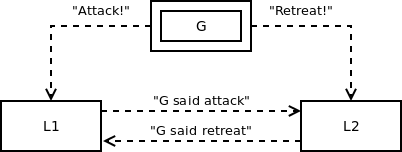
\includegraphics[scale=0.75]{\rootdir/fault-tolerant-design/figures/byzantine-3-party-general-traitor}
\end{center}

\vfill

\begin{center}
  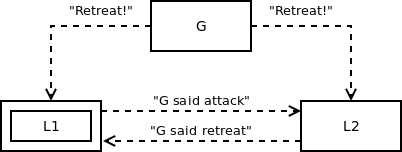
\includegraphics[scale=0.75]{\rootdir/fault-tolerant-design/figures/byzantine-3-party-l2-traitor}
\end{center}

\vfill

\begin{center}
\begin{tabular}{llll}
 \hline
  & \multicolumn{3}{c}{{\bf Received by}}\\
 \cline{2-4}
  {\bf Sent by}  & L1 & L2 & L3\\
\hline
 G & attack & attack & retreat \\
 L\(_1\) & - & attack & attack \\
 L\(_2\) & attack & - & attack \\
 L\(_3\) & retreat & retreat & - \\
 \hline
{\bf Majority vote} & attack & attack & attack\\
 \hline
\end{tabular}~~~~~
\begin{tabular}{llll}
 \hline
  & \multicolumn{3}{c}{{\bf Received by}}\\
 \cline{2-4}
  {\bf Sent by}  & L1 & L2 & L3\\
\hline
 G & attack & attack & attack \\
 L\(_1\) & - & m$_1$ & m$_2$ \\
 L\(_2\) & attack & - & attack \\
 L\(_3\) & attack & attack & - \\
 \hline
{\bf Majority vote} & attack & attack & attack\\
 \hline
\end{tabular}
\end{center}

\vfill

\pagebreak

\begin{quote}
Algorithm \(Byz(0)\)\\
\begin{enumerate}
\setlength{\itemsep}{0pt}\setlength{\topsep}{0pt}

\item The commander sends his orders to every lieutenant.

\item The lieutenant uses the order they receive from the commander or
the default (say retreat) if no order is received. 

\end{enumerate}

Algorithm \(Byz(n)\)\\
\begin{enumerate}
\setlength{\itemsep}{0pt}\setlength{\topsep}{0pt}

\item The commander sends his orders to every lieutenant. 

% Let \(v_i\) be the order sent to lieutenant \(L_i\).

\item For each \(i \in 1.. n\), lieutenant \(L_i\) acts as the general in a \(Byz(n-1)\) algorithm and sends out order \(v_i\) to each of the other \((n-2)\)  lieutenants, i.e.\ \((n-2)\) attempts to agree on \(L_i\ 's\) order.

\item For each \(i\) and \(j \not = i\), let \(w_{ij}\) be the order
that lieutenant \(L_i\) receives from lieutenant \(L_j\) in step 2
(using the \(Byz(n-1)\) algorithm), or the default if no order is
received.  Lieutenant \(L_i\) follows the majority \(\{v_i,
w_{i,j}|i\not = j\}\).

\end{enumerate}

\end{quote}

\pagebreak

\begin{center}
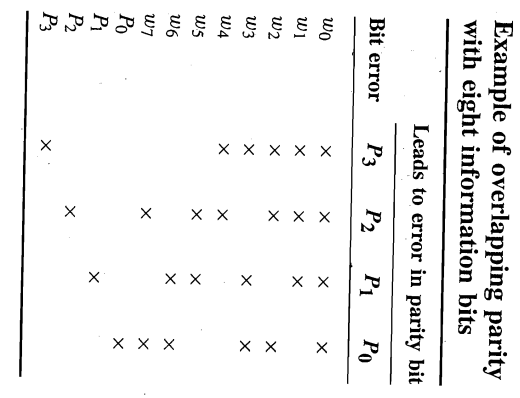
\includegraphics[scale=0.6,angle=91]{\rootdir/fault-tolerant-design/figures/extended-parity-coding}
\end{center}

\end{document}  

% LocalWords:  init PreFill PostFill FillOK GSM de Franche
